\documentclass[11pt,a4paper]{article}

% ---------- Packages ----------
\usepackage[utf8]{inputenc}
\usepackage[T1]{fontenc}
\usepackage{lmodern}
\usepackage{amsmath,amssymb}
\usepackage{enumitem}
\usepackage{geometry}
\usepackage{fancyhdr}
\usepackage[most]{tcolorbox}   % enhanced, breakable
\usepackage{hyperref}

% ---------- Geometry ----------
\geometry{margin=2.5cm}

% ---------- Header/Footer ----------
\setlength{\headheight}{14pt}  % fancyhdr warning verhindern
\pagestyle{fancy}
\fancyhf{}
\lhead{Introduction to Electrical Engineering}
\rhead{Winter Term 2025}
\cfoot{\thepage}

% ---------- Exercise Environment ----------
\newcounter{exercise}
\newenvironment{exercise}[1][]
  {\refstepcounter{exercise}%
   \begin{tcolorbox}[enhanced, breakable, width=\textwidth,
     colback=blue!5!white,colframe=blue!60!black,
     fonttitle=\bfseries\large,
     title=Exercise~\theexercise:~#1]}
  {\end{tcolorbox}}

% ---------- Solution Environment ----------
\newif\ifshowsolutions
\showsolutionstrue  % comment to hide solutions

\newenvironment{solution}
  {\ifshowsolutions
     \begin{tcolorbox}[enhanced, breakable, width=\textwidth,
       colback=green!5!white,colframe=green!50!black,
       fonttitle=\bfseries\large,
       title=Solution]}
  {\end{tcolorbox}\fi}

% ---------- Document ----------
\begin{document}

% ----- Header Box -----
\begin{tcolorbox}[enhanced, breakable, colback=gray!10!white,
  colframe=gray!70!black, fonttitle=\bfseries\large,
  title={Exercise Sheet \#4}: Electric Field]
\begin{center}
  Discussion: Nov 12, 2025
\end{center}
\end{tcolorbox}
\vspace{1cm}

% ----- Exercise 1 -----
\begin{exercise}[Discrete Charge Distribution]
Two point charges of $+3.0\, \mu\mathrm{C}$ each are located at the points $(x, y) = (0, 2.0\, \mathrm{m})$ and $(x, y) = (0, -2.0\, \mathrm{m})$. Two additional point charges, each with charge $q$, are located at $(x, y) = (4.0\, \mathrm{m}, 2.0\, \mathrm{m})$ and $(x, y) = (4.0\, \mathrm{m}, -2.0\, \mathrm{m})$. The electric field at the point $(x, y) = (0, 0)$ due to the four charges is $\vec{E} = (4.0 \cdot 10^{3}~\hat{x})~\mathrm{N/C}$. Determine the value of $q$.
\end{exercise}

\ifshowsolutions
\begin{solution}
The electric field at the origin due to a point charge $Q$ at position $(x, y)$ is given by
\[
\vec{E} = \frac{1}{4\pi \varepsilon_0} \frac{Q}{r^2} \, \hat{r},
\]
where $\hat{r}$ is the unit vector pointing from the charge to the field point.

For the two charges at $(0, 2~\mathrm{m})$ and $(0, -2~\mathrm{m})$, the electric field components at the origin point along the $y$-axis. Since they are equal in magnitude and opposite in direction, they cancel each other:
\[
E_y = 0 \quad \text{(net field from the two $3.0\, \mu\mathrm{C}$ charges)}
\]

The distance to the origin of each $q$ charge is
\[
r = \sqrt{(4.0)^2 + (2.0)^2}\, \mathrm{m} = \sqrt{20}\, \mathrm{m},
\]
and the electric field at the origin due to one $q$ charge has magnitude
\[
E_q = \frac{1}{4\pi\varepsilon_0} \frac{|q|}{r^2}.
\]

At the origin, the $y$-components of the fields from the charges at $(4\, \mathrm{m}, 2\, \mathrm{m})$ and $(4\, \mathrm{m}, -2\, \mathrm{m})$ cancel, while the $x$-components add.

Thus, the total field at the origin due to both $q$ charges is
\[
|E_x| = 2 \cdot E_q \cos\theta,
\]
where $\cos\theta = \frac{x}{r} = \frac{4}{4.472} = 0.894$.

Given that the total field at the origin is 
\[
E_x = 4.0 \cdot 10^3\, \mathrm{N/C},
\]
we have
\[
q = -\frac{E_x \cdot 4\pi\varepsilon_0 \cdot r^2}{2 \cdot \cos\theta} = -\frac{4.0 \cdot 10^3 \cdot 2\pi \cdot 8.854 \cdot 10^{-12} \cdot 20}{0.894}\, \mathrm{C} = -5.0\, \mu\mathrm{C}.
\]
\end{solution}
\fi

% ----- Exercise 2 -----
\begin{exercise}[Electric Displacement]
...
\end{exercise}

\ifshowsolutions
\begin{solution}
...
\end{solution}
\fi

% ----- Exercise 3 -----
\begin{exercise}[Gauss‘s Law]
...
\end{exercise}

\ifshowsolutions
\begin{solution}
...
\end{solution}
\fi

% ----- Exercise 4 -----
\begin{exercise}[DC Steady State]
Find the voltages across the capacitors in the circuit below under DC conditions.

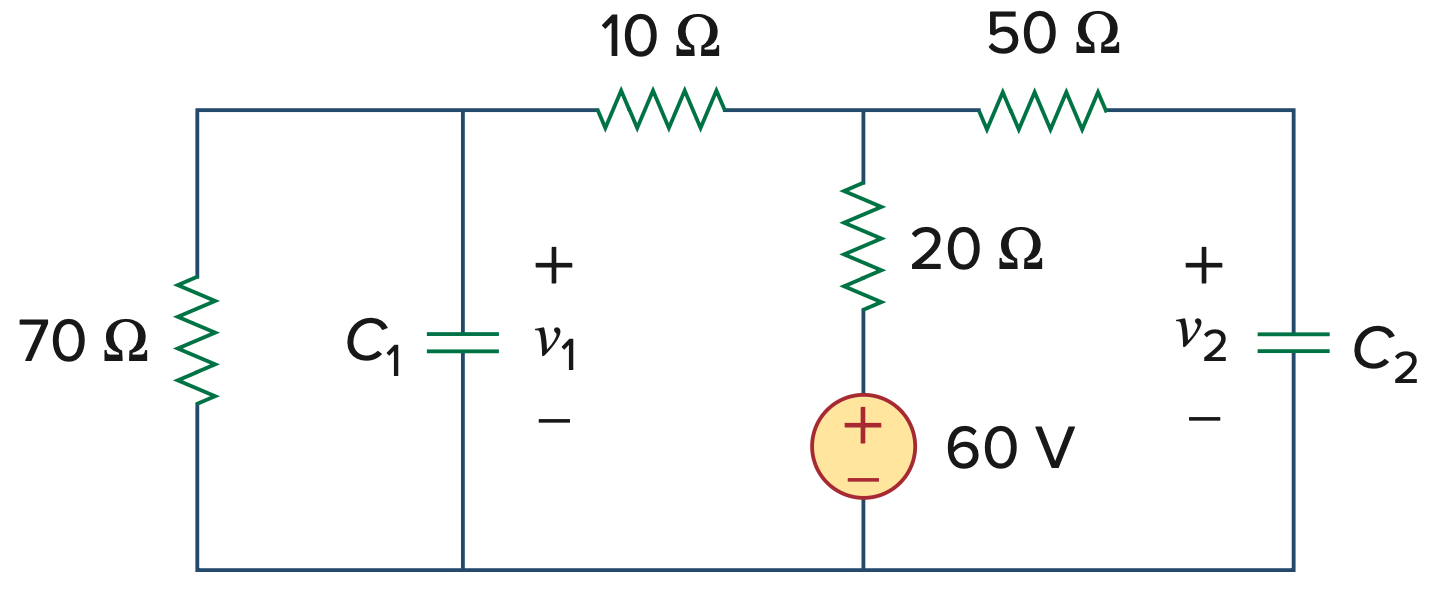
\includegraphics[width=0.7\textwidth]{figures/capacitors.png}
\end{exercise}

\ifshowsolutions
\begin{solution}
Under DC steady-state conditions, the capacitors act as open circuits.  
Therefore, no current flows through \( C_1 \) or \( C_2 \), and we can analyze only the resistive network.

Let the bottom node be the reference (0 V).  
The voltage at the top of the \( 60\text{ V} \) source is \( V_C = 60\text{ V} \).  
Let \( V_A \) and \( V_B \) be the node voltages at the top of \( C_1 \) and the junction between the \( 10\:\Omega \), \( 20\:\Omega \), and \( 50\:\Omega \) resistors, respectively.

\[
\text{KCL at node } A: \quad \frac{V_A - 0}{70} + \frac{V_A - V_B}{10} + I_{C_1} = 0
\]
\[
\Rightarrow \frac{V_A - 0}{70} + \frac{V_A - V_B}{10} = 0
\]

\[
\text{KCL at node } B: \quad \frac{V_B - V_A}{10} + \frac{V_B - 60}{20} + I_{C_2} = 0
\]
\[
\Rightarrow \frac{V_B - V_A}{10} + \frac{V_B - 60}{20} = 0
\]

Multiply the first equation by \(70\):
\[
V_A + 7(V_A - V_B) = 0 \quad \Longrightarrow \quad 8V_A - 7V_B = 0
\]

Multiply the second equation by \(20\):
\[
2(V_B - V_A) + (V_B - 60) = 0 \quad \Longrightarrow \quad -2V_A + 3V_B = 60
\]

Substitute into each other:
\[
-2\left(\frac{7}{8}V_B\right) + 3V_B = 60
\]

\[
\Rightarrow \left(-\frac{14}{8} + \frac{24}{8}\right)V_B = 60
\]

\[
\Rightarrow V_B = 60 \cdot \frac{8}{10} = 48~\text{V}
\]

\[
V_A = \frac{7}{8}V_B = \frac{7}{8} \cdot 48 = 42~\text{V} = v_1
\]

Finally, let \( V_D \) be the trivial node (just one input and one output) voltage between the top of \( C_2 \) and the \( 50\:\Omega \) resistor.
\[
\text{KCL at node } D: \quad \frac{V_D - V_B}{50} + I_{C_2} = 0 
\]
\[
I_{C_2} = 0 \; (\text{DC steady state}) 
\;\Rightarrow\; \frac{V_D - V_B}{50} = 0 
\;\Rightarrow\; V_D = V_B
\;\Rightarrow\; v_2 = V_B
\]

\[
\boxed{v_1 = 42~\text{V}, \quad v_2 = 48~\text{V}}
\]
\end{solution}
\fi

% ----- Exercise 5 -----
\begin{exercise}[Plate Capacitor]
...
\end{exercise}

\ifshowsolutions
\begin{solution}
...
\end{solution}
\fi

% ----- Exercise 6 -----
\begin{exercise}[...]
...
\end{exercise}

\ifshowsolutions
\begin{solution}
...
\end{solution}
\fi

% ----- Exercise 7 -----
\begin{exercise}[...]
...
\end{exercise}

\ifshowsolutions
\begin{solution}
...
\end{solution}
\fi

% ----- Exercise 8 -----
\begin{exercise}[...]
...
\end{exercise}

\ifshowsolutions
\begin{solution}
...
\end{solution}
\fi

\end{document}